\section{\name Rollback Protection}
\label{sec:rollback}

%In the previous sections, we explain how \name users proximity to achieve identity and location-based attestation for Intel SGX processor. In this section we show that using these primitives, we can achieve even stronger security guarantee for SGX. We call this to be \emph{Platform Integrity} where the single \device not only provides enhanced attestation but also ensures the hardware integrity of the system. One of the most susceptible components towards hardware manipulation is the mass storage drive. Intel SGX provides the sealing mechanism to prevent the integrity of the data. But the integrity of the drive is not ensured. 


In this section, we address the third listed limitation of SGX: rollback protection. The problem is simple to solve, if a secure and performant counter service is available to enclaves. An external embedded device can easily support the needed non-volatile storage for counters, but the real challenge is how to establish secure communication between the enclave and this device. While such devices can be certified so that enclaves only connect to devices from a trusted issuer, an attacker that controls the OS can relay the initial connection establishment from the enclave to another certified device that the attacker has physical access to and can attack much easier. The enclave cannot distinguish one certified device from another.

We propose a solution that prevents such relay attacks by performing proximity verification in the reverse direction. That is, in this use case the enclave establishes a secure connection to an attached embedded device and verifies its proximity.  

%The embedded device provides a simple API that consists of three functions. First, \texttt{createCounter()} creates a new counter and returns a random identifier (\texttt{ID}) for it. Second, \texttt{readCounter(ID)} returns the value of the requested counter. And third, \texttt{incCounter(ID)} increments a counter. Using these functions, enclaves can secure seal and unseal data. 

%There are two ways the enclave can invoke \getcounter, either \getcounter where the \device initializes a new monotonic counter and returns a new randomly generated identifier (of sufficiently large length) to which the counter is mapped to or \getcounterID{ID} where the enclave provides the identifier \texttt{ID} and the \device returns the current counter value. Every \getcounter value causes an increment of the corresponding counter value. Note, that the identifier is a secret value here which is required to access the counter.  
 
%\begin{figure}[t]
% \centering
% %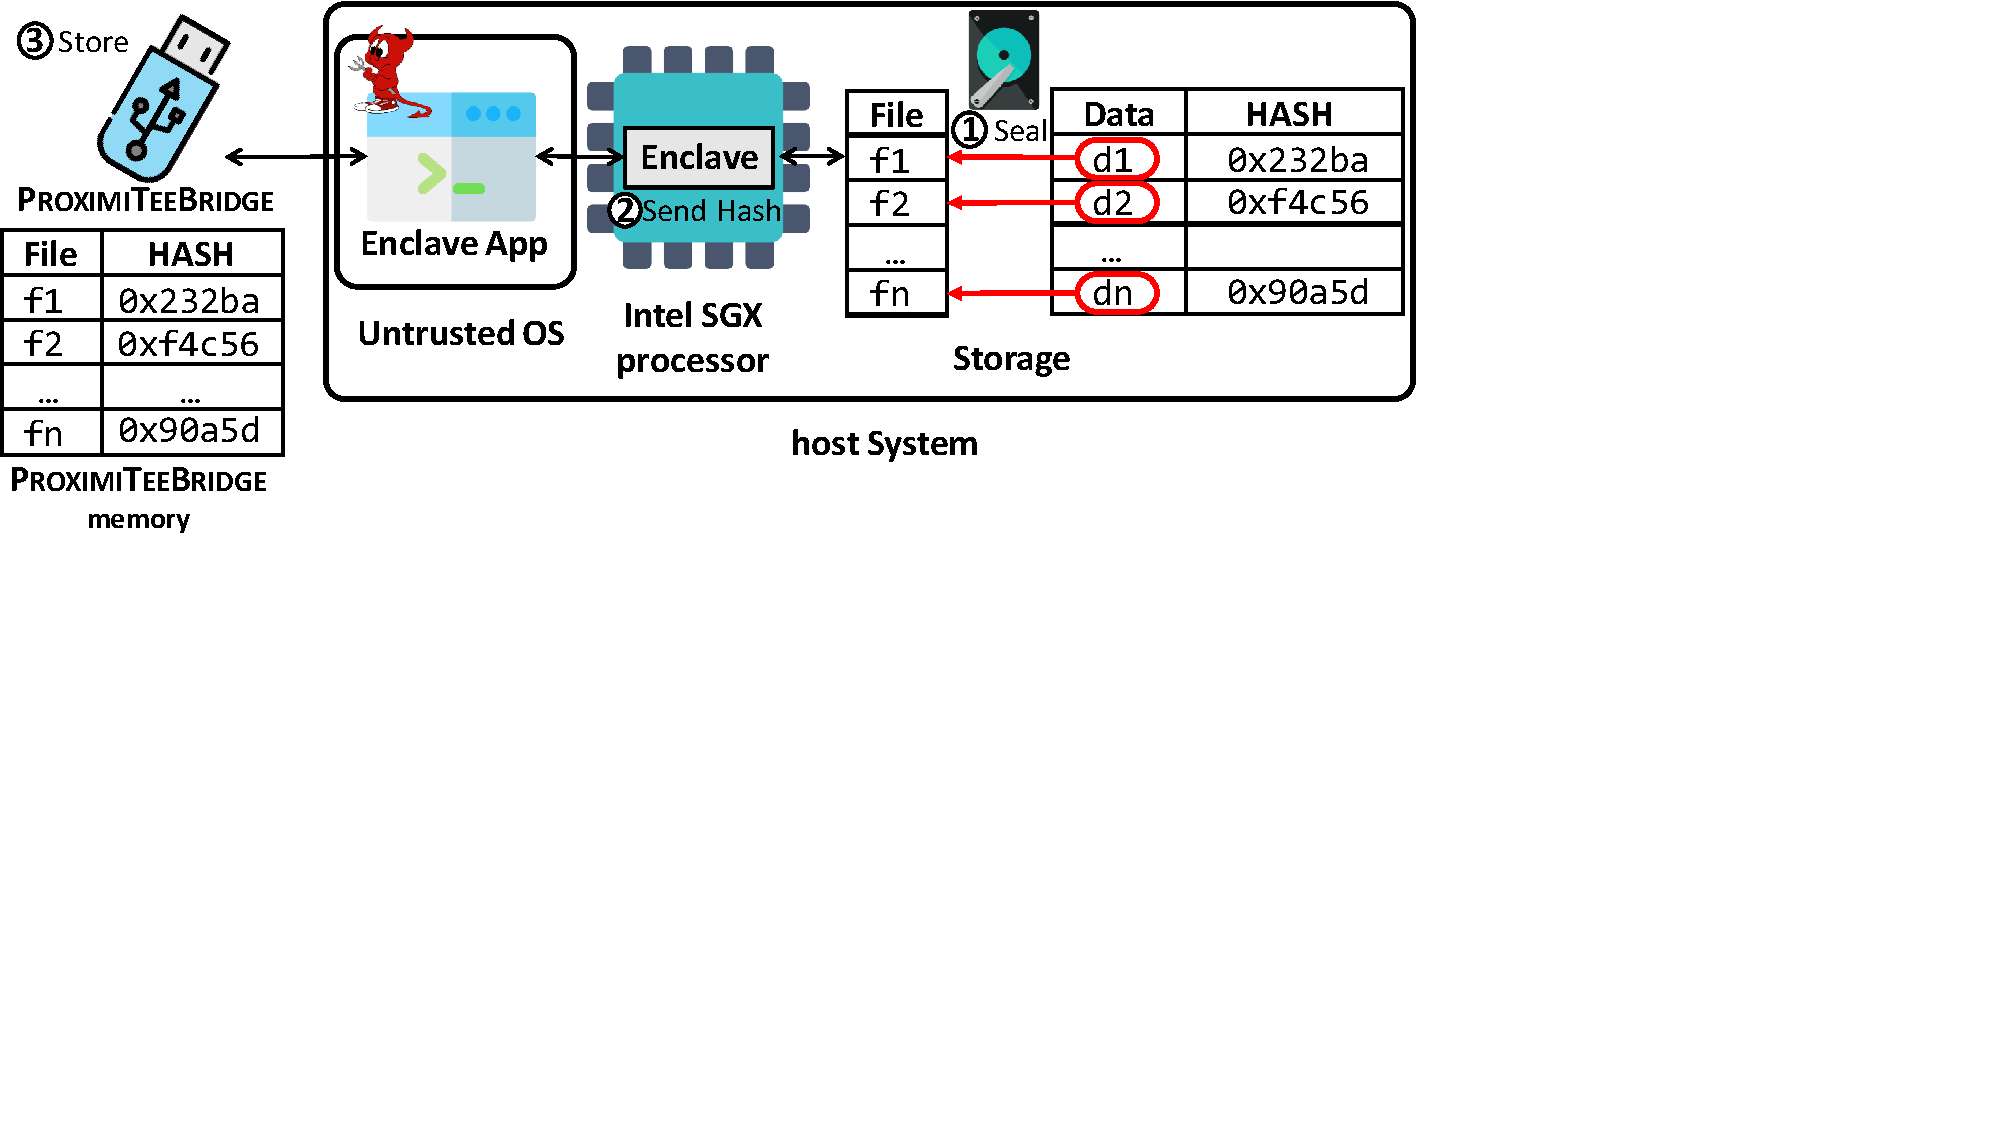
\includegraphics[trim={0 10cm 9cm 0},clip,width=0.85\linewidth]{RollBack.pdf}
% 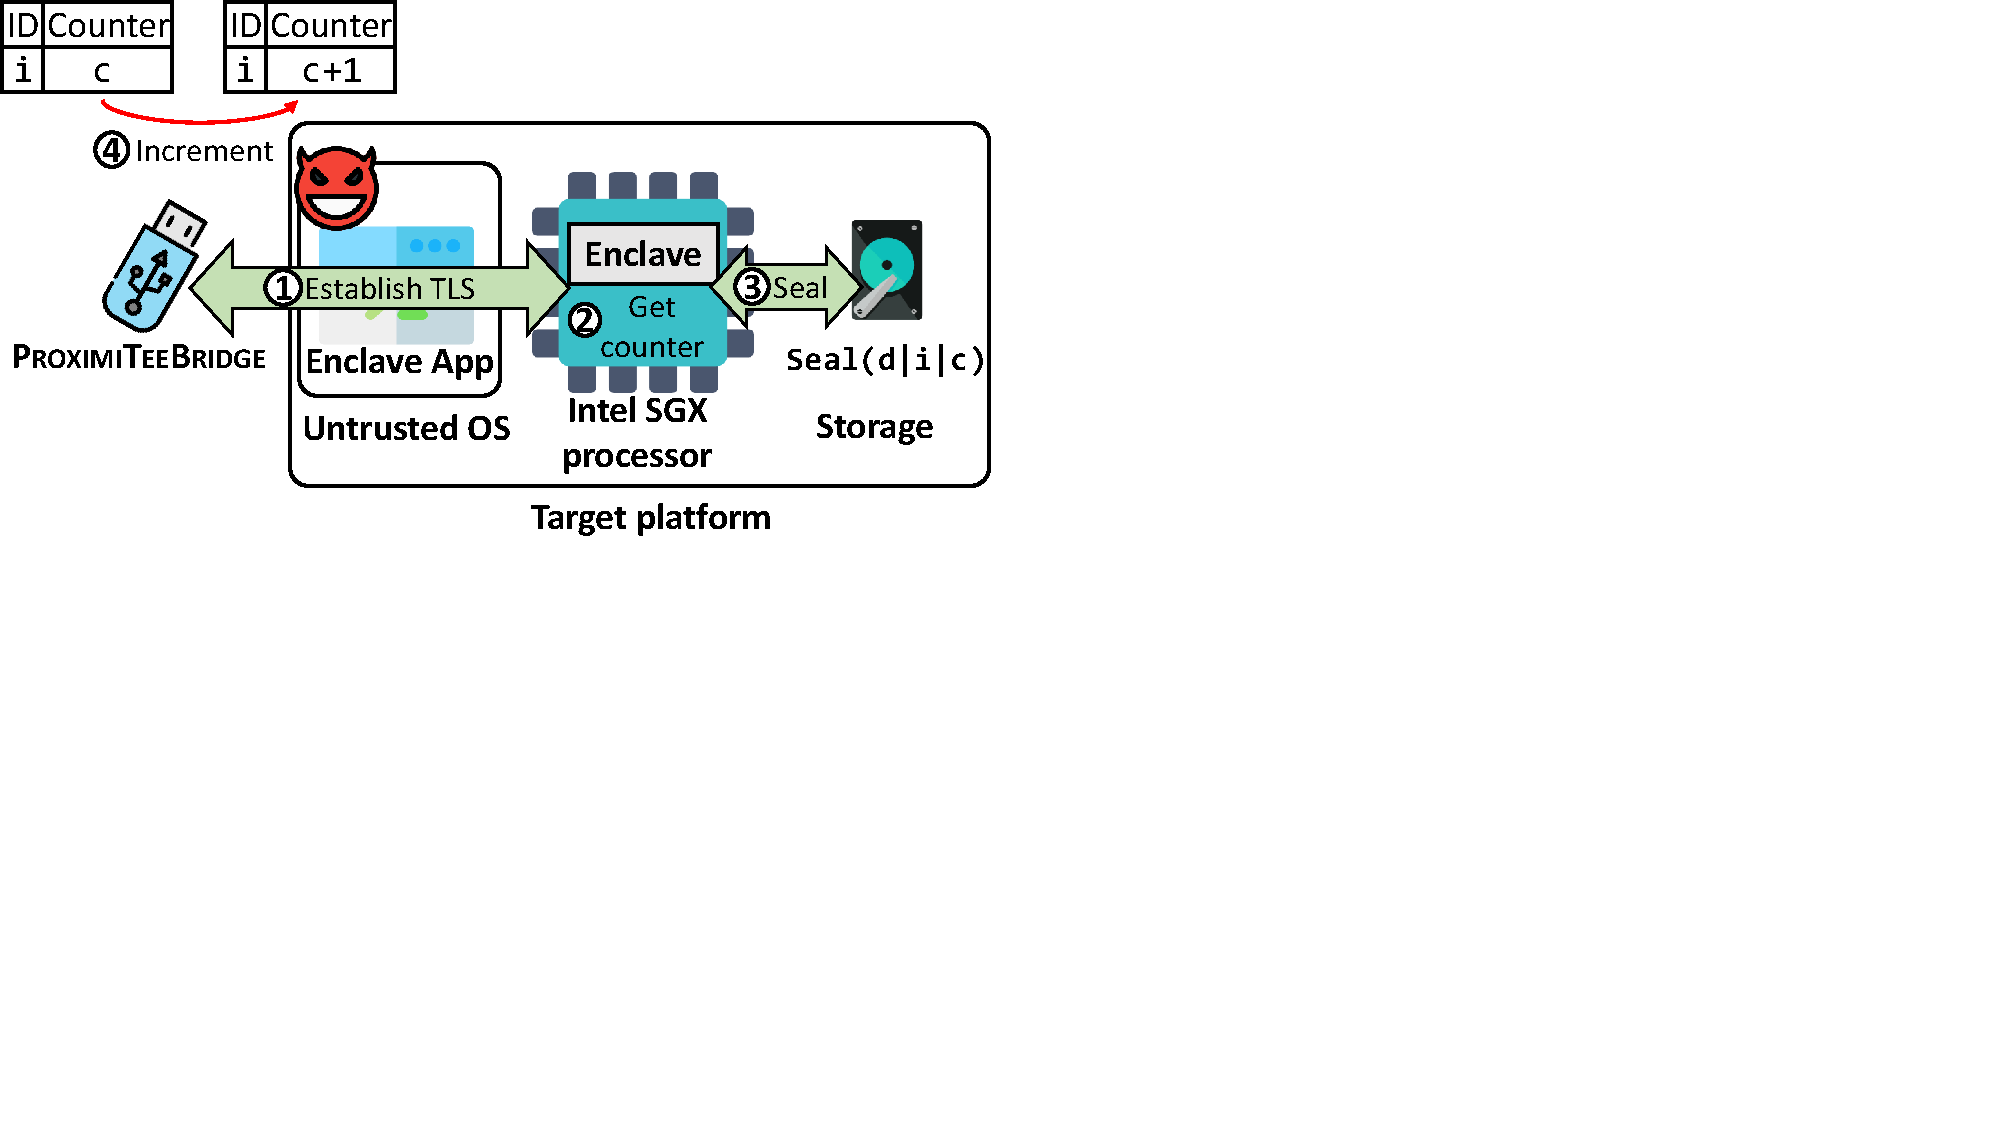
\includegraphics[trim={0 10cm 16cm 0},clip,width=\linewidth]{RollBack_revised.pdf} 
% \caption{\emph{Rollback protection.} Enclave communicates securely with the \device and execute enclave-side \name protocol to determine the proximity of the \device. The \device has a non-volatile flash memory where it keeps the monotonic counter that is used by the enclave for sealing which in turn protects against rollback attack.}
% \label{fig:rollback}
%\end{figure}


\myparagraph{Initialization.} The initialization phase is executed only once that allows the \device and the enclave to establish a \tls channel. Additionally, the enclave also executes the enclave-side challenge-response protocol. The protocol ensures that the enclave is communicating with a legitimate \device (signed by the valid manufacturer) that is connected to the platform physically (over \usb interface). If the challenge-response protocol returns a negative response, the enclave aborts. After the successful \name protocol, the enclave and the \device acquires others' public keys. During sealing and unsealing process, the enclave and the \device establishes a \tls channel using these keys. 

\myparagraph{Sealing and unsealing.} Once a secure connection to the embedded device is created, the embedded device can provide a simple counter service that the enclave can use for rollback protection. 

Two common techniques for counter-based rollback protection exist~\cite{matetic2017rote}. The first technique is \emph{inc-then-store}, where the enclave first increments the trusted counter (on the embedded device) and after that updates its internal state and stores the sealed state together with the counter value on disk. This approach provides a strong security property (no rollback to any previous state), but if the enclave crashes between the increment and store operations, the system cannot recover from the crash.

The second technique is \emph{store-then-inc}, where the enclave first saves its state on the disk together with the latest input value, after that increments the trusted counter (on the embedded device), and finally performs the state update~\cite{ice, memoir}. If the system crashes, it can recover from the previous state using the saved input. This technique requires a deterministic enclave and provides a slightly weaker security property: arbitrary rollback is not possible, but the last input may be executed twice on the same enclave state~\cite{memoir}.


%\myparagraph{Sealing.} The sealing process is illustrated in Figure~\ref{fig:rollback} and it proceeds as follows: 
%
%\begin{enumerate} [leftmargin=*]
%  \item The \device establishes a \tls channel with the enclave using public keys aquired from the initialization phase.
%  \item The enclave requests a counter value (\getcounter) from the \device. If the enclave is sealing a new data, it invokes \texttt{createCounter()} which returns a new counter value \texttt{c} and corresponding identifier \texttt{ID}. 
%  \item The enclave seals \texttt{(data|ID|c)} in the mass storage. 
%  \item Along with the \getcounter call, the enclave also invoke \texttt{incCounter(ID)} that cause the \device to increment the counter value corresponding to the identifier by one. In case the enclave is re-sealing older data, the enclave first unseals the data, get the identifier \texttt{ID} and invoke \getcounterID{ID}.
%\end{enumerate}
%
%
%\myparagraph{Unsealing.} Unsealing happens as follows:
%
%\begin{enumerate}[leftmargin=*]
%  \item The enclave first unseals the sealed data and recover \texttt{(data|ID|c)} from the mass storage device.
%  \item The enclave invokes \getcounterID{ID} over the \tls channel to the \device. If the \device contains \id, it returns the corresponding counter value $\texttt{c}'$. If the \device does not have the \id registered on its non-volatile memory, it returns an error. If the enclave receives an error, it concludes that the sealed data is corrupted.
%  \item If the enclave receives a valid counter value $\texttt{c}'$, it checks if $\texttt{c}=\texttt{c'}$. If the check fails, the enclave concludes that a rollback attack took place and throws an error.
%\end{enumerate}



